\begin{frame}{Teorema Principal}
    \begin{thm}[1 \cite{Baker83}] \label{teo1}
            Existe um PTAS para CI em grafos planares, com tempo $O(2^{O(\nicefrac{1}{\varepsilon})} \cdot n)$.
        \end{thm}
\end{frame}

\begin{frame}{Observação}
    \centering
    \vspace{1cm}
    \pause
    \Large Assim como ogros, grafos planares têm camadas!
    \begin{minipage}{\linewidth}
        \centering
        \vspace{1.73cm}
        
\includegraphics[height=5cm]{images/shrek.png}
    \end{minipage}
\end{frame}

\begin{frame}{Exemplo}
    \begin{minipage}{\linewidth}
        \centering
        \only<1>{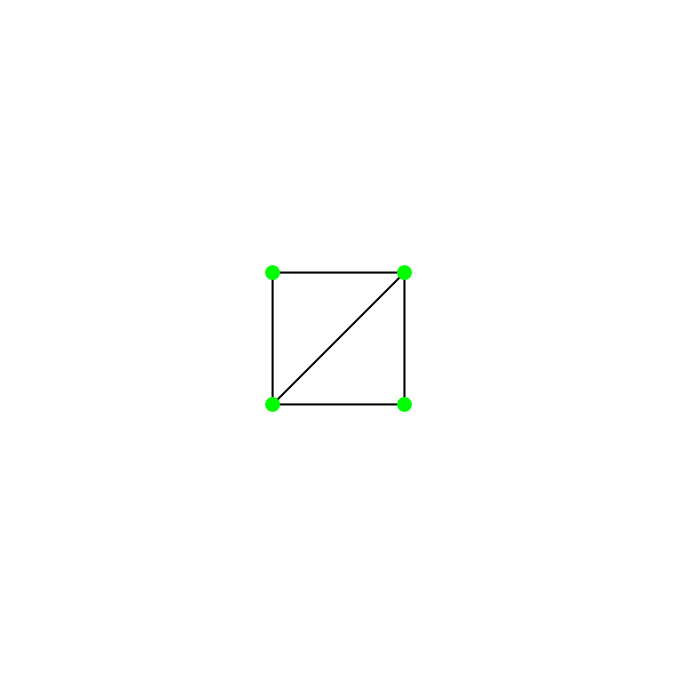
\includegraphics[height=6cm]{images/outer1.png}}
        \only<2>{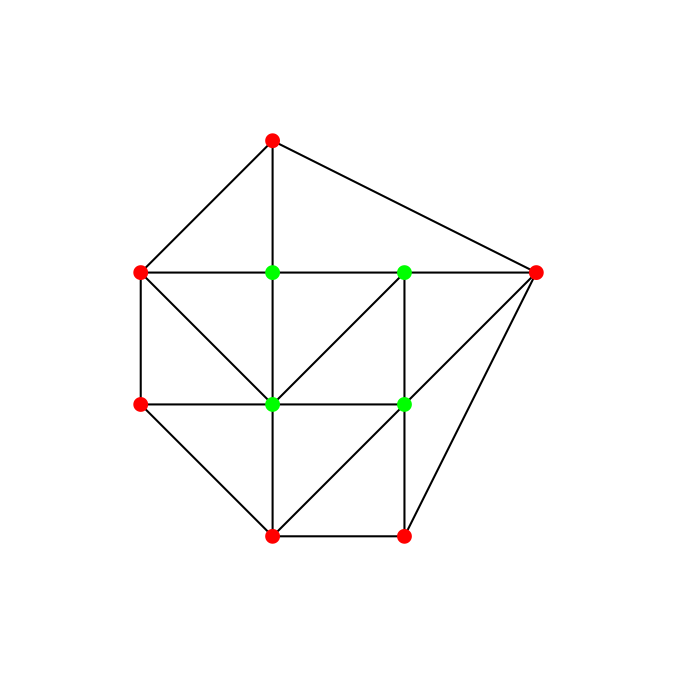
\includegraphics[height=6cm]{images/outer2.png}}
        \only<3>{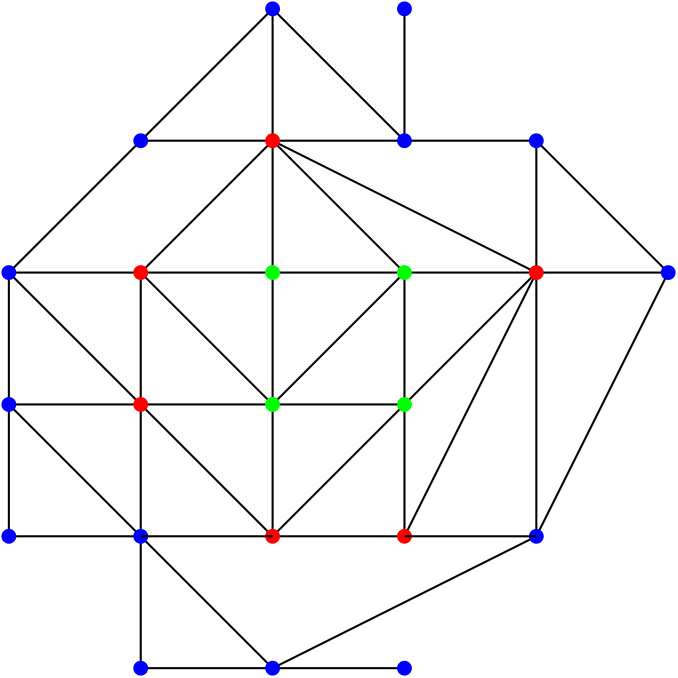
\includegraphics[height=6cm]{images/outer3.png}}
    \end{minipage}
\end{frame}

\begin{frame}{Preparação}
    Dado $G=(V, E)$ planar e $\varepsilon > 0$, definimos:
    \pause
    \begin{enumerate}[-]
        \item $k=\ceil{\nicefrac{1}{\varepsilon}}$;
        \item Para $0 \le i < k$, seja $S_i = \{L_j \mid j \equiv i \pmod k\}$
        \begin{enumerate}[-]
            \item Ex.: $k = 4 \Rightarrow S_1 = L_1 \cup L_5 \cup L_9 \cup \dots$
        \end{enumerate}
        \item $G_i = G[V - S_i]$.
    \end{enumerate}
\end{frame}

\begin{frame}{Decomposição em \emoji{onion}}
    \centering
    \Large $k=3$:
    \bigbreak
    \begin{minipage}{\linewidth}
        \centering
        \only<1>{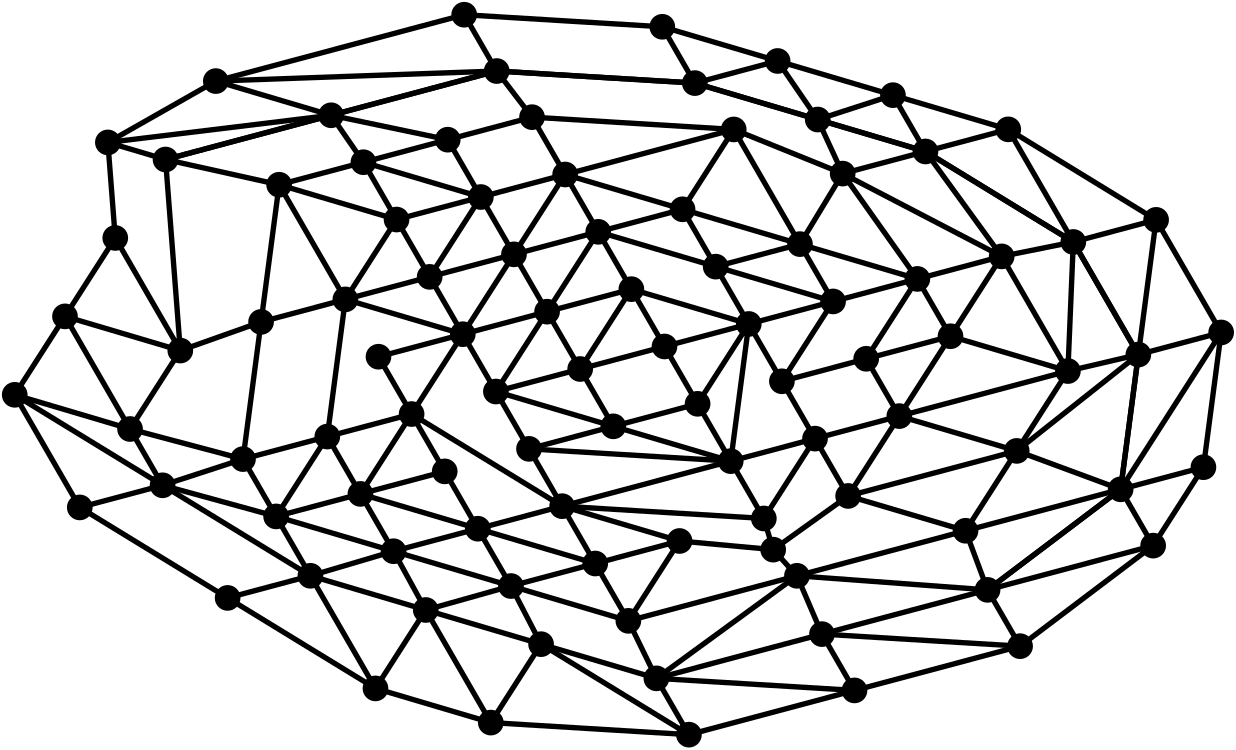
\includegraphics[height=5cm]{images/onion1.png}}
        \only<2>{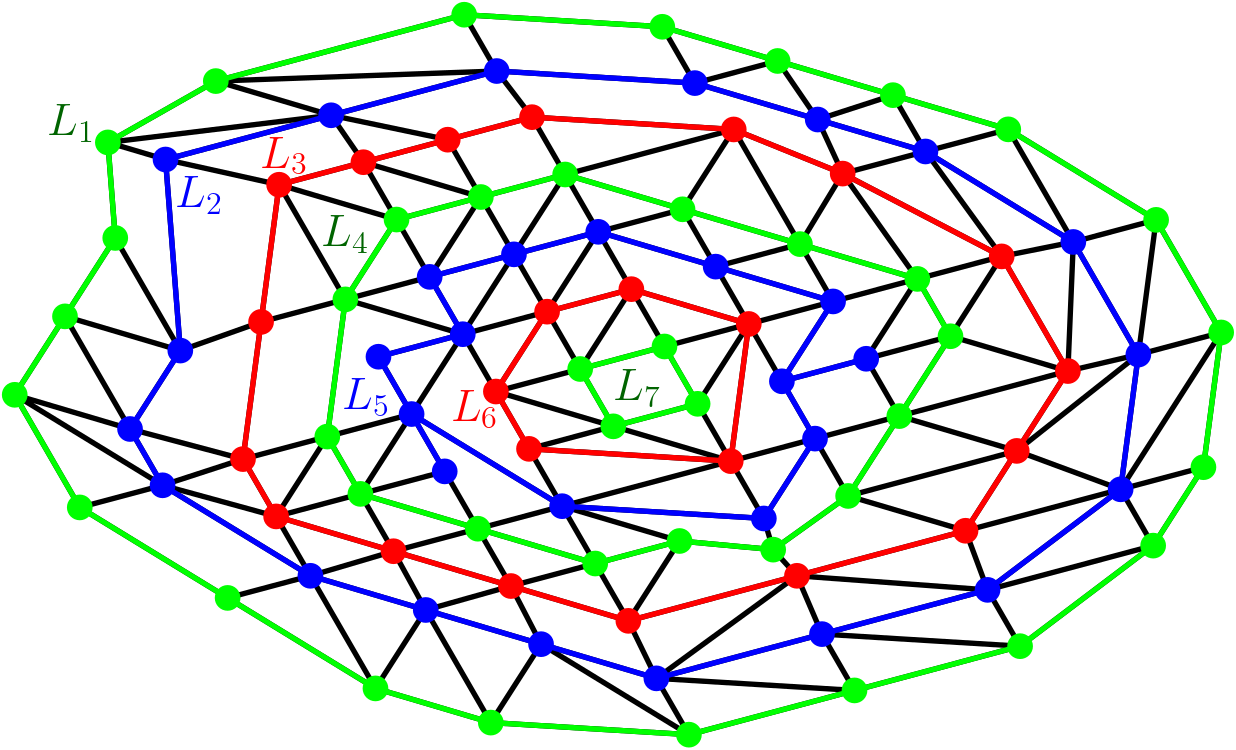
\includegraphics[height=5cm]{images/onion2.png}}
        \only<3>{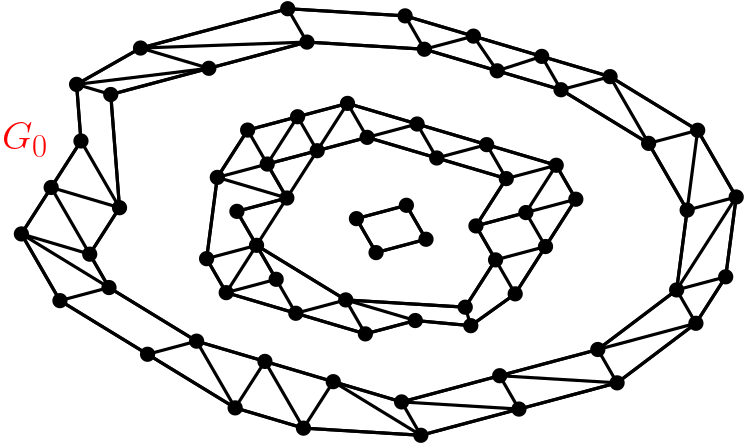
\includegraphics[height=5cm]{images/onion3.png}}
        \only<4>{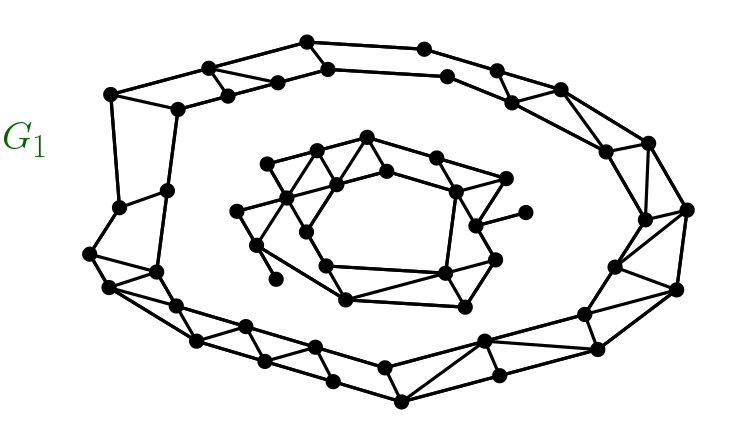
\includegraphics[height=5cm]{images/onion4.png}}
        \only<5>{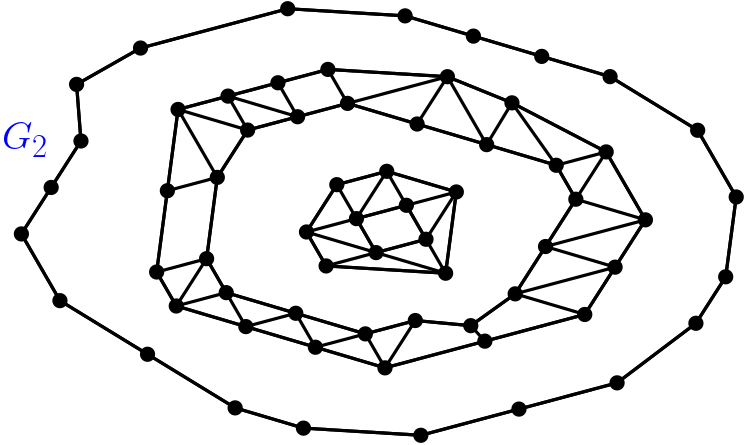
\includegraphics[height=5cm]{images/onion5.png}}
    \end{minipage}
\end{frame}

\begin{frame}{Solucionando $G_i$}
    \centering\Large
    Aplicamos o Lema \ref{lema1} em cada componente.
\end{frame}

\begin{frame}{Solução Ótima para $G_i$}
    \centering\Large
    Para cada $i$, geramos uma solução ótima $X_i$ de $G_i$.
    \bigbreak
    O tempo total gasto é $2^{O(k)} \cdot n = 2^{O(\nicefrac{1}{\varepsilon})} \cdot n$.
\end{frame}

\begin{frame}{Aproximação para $G$}
    \centering\large
    Basta retornar o $X_\alpha$ de maior cardinalidade!
\end{frame}

\begin{frame}{Fator de Aproximação}
    \pause
    \setbeamercovered{transparent} % fade-in/fade-out lists
    \begin{proof}
        \begin{enumerate}
            \setlength\itemsep{1em}
            \item<2,8> Seja $O \subseteq V$ uma solução ótima;
            \item<3,8> $S_0, \dots, S_{k-1}$ particionam $V$;
            \item<4,8> Algum $i$ satisfaz $|O \cap S_i| \leq \nicefrac{|O|}{k}$;
            \item<5,8> $O \setminus S_i$ é independente em $G_i$;
            \item<6,8> Então $|X_\alpha| \ge |O \setminus S_i| = |O| - |O \cap S_i|$;
            \item<7,8> Portanto, $|X_\alpha| \ge \left(1 - \frac{1}{k}\right)|O| \ge (1 - \varepsilon) \cdot OPT$.
        \end{enumerate}
        \alt<8>{\qedhere}{\phantom\qedhere}
    \end{proof}
\end{frame}
